\chapter{Laplace's Equation}

\todo[inline]{Show that classical solutions are not always available}
\todo[inline]{Show the derivation of the weak form}
\todo[inline]{Discretise the domain and show how we represent functions there}
\todo[inline]{Show how to construct the FEM linear system}

Our problem concerns the following partial differential equation:

\begin{align}\label{eq:general_laplace}
    \generalLaplaceEqn \text{, in } \Omega \\
    u &= 0 \text{, on } \partial\Omega = \Gamma
\end{align}

In order to apply the finite element method, we need to obtain the weak
formulation of the above equation.

So for $v \in V$:

\[
    \int_{\Omega}{v(\nabla\cdot(a\nabla{u}))}\,d\Omega +
    \int_{\Omega}\v{b}\cdot v\nabla{u}\,d\Omega +
    \int_{\Omega}cuv\,d\Omega = \int_{\Omega}fv\,d\Omega
\]

Applying Green's first integral identity to the first term we get:

\[
    \int_{\Omega}a\nabla{v}\cdot\nabla{u}\,d\Omega -
    \int_{\Gamma}av
      \underbrace{\frac{\partial{u}}{\partial{n}}}_{=0}
      \,d\Gamma +
    \int_{\Omega}\v{b}\cdot v\nabla{u}\,d\Omega + \int_{\Omega}cuv\,d\Omega =
    \int_{\Omega}fv\,d\Omega
\]

As per our boundary conditions $u=0$ on $\Gamma$ which caues the second
integral to vanish hence:

\[
    \int_{\Omega}a\nabla{v}\cdot\nabla{u}\,d\Omega +
    \int_{\Omega}\v{b}\cdot v\nabla{u}\,d\Omega + \int_{\Omega}cuv\,d\Omega =
    \int_{\Omega}fv\,d\Omega
\]

Then if we define our bilinear form to be:

\[
    a(u,v) =
    \int_{\Omega}a\nabla{v}\cdot\nabla{u}\,d\Omega +
    \int_{\Omega}\v{b}\cdot v\nabla{u}\,d\Omega + \int_{\Omega}cuv\,d\Omega
\]

and the linear functional to be:

\[
    l(v) = \int_{\Omega}fv\,d\Omega
\]

Then we have a weak solution when we can find $u \in V$ such that:

\begin{equation}\label{eq:weak_formulation}
    a(u,v) = l(v)\, \forall v \in V
\end{equation}

\section{Discretising the domain}

We divide each $[0,1]$ interval into $N$ segments of length $h = \frac{1}{N}$ 
which we can use to subdivide the domain into a grid. Placing a node $x_{ij}$ at 
each intersection of the grid lines gives us $(N + 1)^2$ nodes which we can use to
to approximate functions on this domain with.

In order to approximate functions on this domain we need to choose an appropriate
basis

From this then  we can construct a uniform triangulation $T_h$ of
$[0,1] \times [0,1]$, see Figure \ref{fig:example_triangulation} for an example 
triangulation of the domain.

\begin{figure}\label{fig:example_triangulation}
\centering
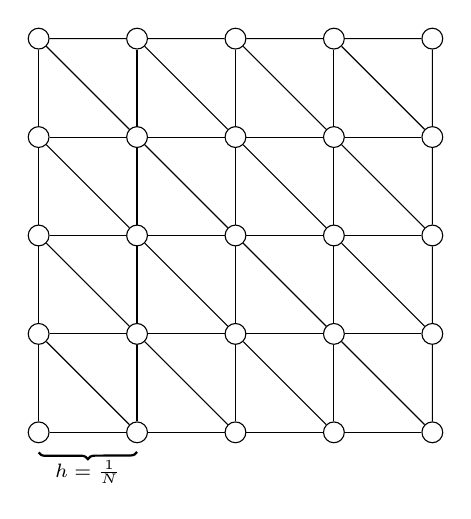
\begin{tikzpicture}[scale=5]

	\scriptsize
	% Place each of the nodes in the grid
	\foreach \x in {0,...,4}
		\foreach \y in {0,...,4}
        	{
               \node[circle,draw=black] 
                         (\x\y) at (0.25*\x,0.25*\y) {};
       		}
            
    % Draw each horizontal line between the nodes
    \foreach \y in {0,...,4}
    	\foreach \x in {0,...,3}
            {
                \pgfmathtruncatemacro{\idx}{\x + 1}
            	\draw (\x\y) -- (\idx\y);
            }
            
    % Draw each vertical line between the nodes
    \foreach \x in {0,...,4}
    	\foreach \y in {0,...,3}
            {
            	\pgfmathtruncatemacro{\idx}{\y + 1}
                \draw (\x\y) -- (\x\idx);
            }
            
     % Finally draw each diagonal to complete the triangulation
     \foreach \y in {1,...,4}
         \foreach \x in {0,...,3}
             {
                \pgfmathtruncatemacro{\xidx}{\x + 1}
                \pgfmathtruncatemacro{\yidx}{\y - 1}
          	    \draw (\x\y) -- (\xidx\yidx);
             }
             
      % Illustrate the length of each segment
      \draw[thick,decoration={brace, mirror}, decorate]
          (0, -0.051) -- (0.25, -0.05)
          node[pos=0.5,anchor=north] {$h = \frac{1}{N}$};
\end{tikzpicture}
\caption{Example triangulation of $\Omega$ with $N = 4$}
\end{figure}



As we will see it will be useful to introduce a mapping that will let us
evaluate integrals for arbitrary triangles by considering a single reference
triangle comprised of the points $(0,0), (0,1), (1,0)$

\todo[inline]{Explain the master triangle, the mapping etc}

\begin{align}\label{eq:master_basis_functions}
    \psi_1(\zeta, \eta) &= 1 - \zeta - \eta \\
    \psi_2(\zeta, \eta) &= \zeta \\
    \psi_3(\zeta, \eta) &= \eta
\end{align}

It will also be useful to consider the derivatives of these functions:

\begin{align}\label{eq:master_basis_functions_derivative}
    \psi_1' = \nabla\psi_1(\zeta, \eta) &=
        \frac{1}{h}\left(\begin{array}{c}-1 \\ -1\end{array}\right) \\
    \psi_2' = \nabla\psi_2(\zeta, \eta) &=
        \frac{1}{h}\left(\begin{array}{c}1 \\ 0\end{array}\right) \\
    \psi_3' = \nabla\psi_3(\zeta, \eta) &=
        \frac{1}{h}\left(\begin{array}{c}0 \\ 1\end{array}\right)
\end{align}

\section{The Local Stiffness Matrix}

Each local stiffness matrix will have dimension $3 \times 3$ and will be given
by:

\begin{align*}
    A^k_{i,j} &= a_k(\phi_j, \phi_i) \\
     &= \int_{T_k}a\nabla\phi_i\cdot\nabla\phi_j\,dxdy +
        \int_{T_k}\v{b}\cdot\phi_j\nabla\phi_i\,dxdy +
        \int_{T_k}c\phi_i\phi_j\,dxdy
\end{align*}

To simplify the integrations we will apply our mapping so that we have:

\[
    A^k_{i,j} = h^2\int_Ta\nabla\psi_i\cdot\nabla\psi_j\,d\zeta d\eta +
                h^2\int_T\v{b}\psi_j\nabla\psi_i\,d\zeta d\eta +
                h^2\int_Tc\psi_i\psi_j\,d\zeta d\eta
\]

Considering each term in isolation:

\[
    ah^2\int_T\nabla\psi_i\cdot\nabla\psi_j\,d\zeta d\eta =
    a\int_T\psi'_{i\zeta}\psi'_{j\zeta} +
        \psi'_{i\eta}\psi'_{i\eta}\,d\zeta d\eta
\]

We can see from this that the resulting matrix will be symmetric, let's
consider the case when $i = 1 = j$:

\begin{align*}
    a\int_T(\psi'_{1\zeta})^2 + (\psi'_{1\eta})^2\,d\zeta d\eta & =
        a\int_T(-1)^2 + (-1)^2\,d\zeta d\eta \\
    &= 2a\int_0^1\int_0^\eta\,d\zeta d\eta \\
    &= 2a\frac{1}{2} \\
    &= a
\end{align*}

Evaluating similar integrals for each entry in the matrix results in the following
local stiffness matrix associated with the Laplacian term:

\begin{equation}\label{eq:stiffness_term_1}
    a\left(\begin{array}{c c c}
        1      & -\half & -\half \\
        -\half & \half  & 0 \\
        -\half & 0      & \half
    \end{array}\right)
\end{equation}

Now let's consider the second term, in the case when $i = 2, j = 1$:

\begin{align*}
    h^2\int_T{\v{b}\psi_1\nabla\psi_2}\, d\zeta d\eta &=
    -h\int_0^1\int_0^\eta{\zeta b_x + \zeta b_y}\, d\zeta d\eta \\
    &= -h(b_x + b_y)\int_0^1\int_0^\eta{\zeta}\, d\zeta d\eta \\
    &= -\frac{h(b_x + b_y)}{6}
\end{align*}

Repeating this for the other entries we get the matrix:

\begin{equation}\label{eq:stiffness_term_2}
    h\left(\begin{array}{c c c}
        -\frac{(b_x + b_y)}{12} & \frac{b_x}{6} & \frac{b_y}{6} \\
        -\frac{(b_x + b_y)}{12} & \frac{b_x}{6} & \frac{b_y}{6} \\
        -\frac{(b_x + b_y)}{12} & \frac{b_x}{6} & \frac{b_y}{6}
    \end{array}\right)
\end{equation}

Finally let's consider the third integral, in the case where $i = j = 1$:

\begin{align*}
       ch^2\int_T{\psi_1\psi_1}\,d\zeta d\eta
       &= ch^2\int_0^1\int_0^\eta{(1 - \zeta - \eta)^2}\, d\zeta d\eta \\
%
       &= ch^2\int_0^1\int_0^\eta\, d\zeta d\eta +
          2ch^2\int_0^1\int_0^\eta{\zeta\eta - \zeta - \eta}\, d\zeta d\eta +
          ch^2\int_0^1\int_0^\eta{\zeta^2 + \eta^2}\, d\zeta d\eta \\
%
       &= \frac{ch^2}{2} - \frac{3ch^2}{4} + \frac{ch^2}{3} \\
       &= \frac{ch^2}{12}
\end{align*}

Following a similar argument for the other entries gives us the following
matrix:

\begin{equation}\label{eq:stiffness_term_3}
    \frac{ch^2}{2}\left(\begin{array}{c c c}
         \frac{1}{12} &  \frac{1}{24} &  \frac{1}{24} \\
         \frac{1}{24} &  \frac{1}{12} &  \frac{1}{24} \\
         \frac{1}{24} &  \frac{1}{24} &  \frac{1}{12}
    \end{array}\right)
\end{equation}

Combining (\ref{eq:stiffness_term_1}), (\ref{eq:stiffness_term_2}),
(\ref{eq:stiffness_term_3}) gives us the local stiffness matrix for the general
form of the equation (\ref{eq:general_laplace})

\section{The Local Mass Matrix}

The local mass matrix will also have dimension $3 \times 3$
